
\section{Placement}
\end{multicols}
{
    \centering
    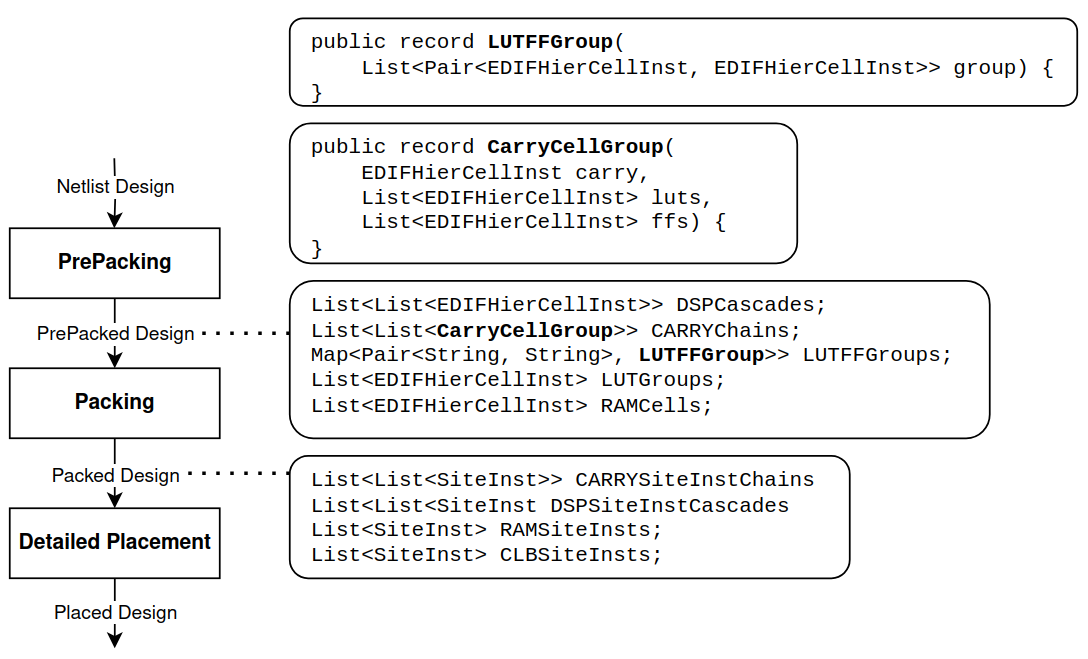
\includegraphics[width=0.8\columnwidth]{figures/substages.png}
    \captionof{figure}{The data classes populated at each substage: \texttt{PrepackedDesign}, \texttt{PackedDesign}, and \texttt{PlacedDesign}.}
    \label{fig:substages}
}
\begin{multicols}{2}
\label{sec:simulated_annealing}
With a basic understanding of FPGA architecture, design placement, and RapidWright, we have all the necessary pieces to implement our SA placer. 
Here we outline in detail each substage of our implementation: PrePacking, Packing, and Placement. 
Shown in Figure \ref{fig:edif_design_device} is an overview of the placement workflow. 
Figure \ref{fig:substages} shows the data structures of RapidWright objects that are populated at each stage: \texttt{PrepackedDesign}, which is a group of data structures around \texttt{EDIFHierCellInst}s, \texttt{PackedDesign}, which is a group fo data structures around \texttt{SiteInst}s, and finally, \texttt{PlacedDesign}, which is simply captured by the final RapidWright \texttt{Design} object. 

\vspace{0.5cm}
{
    \centering
    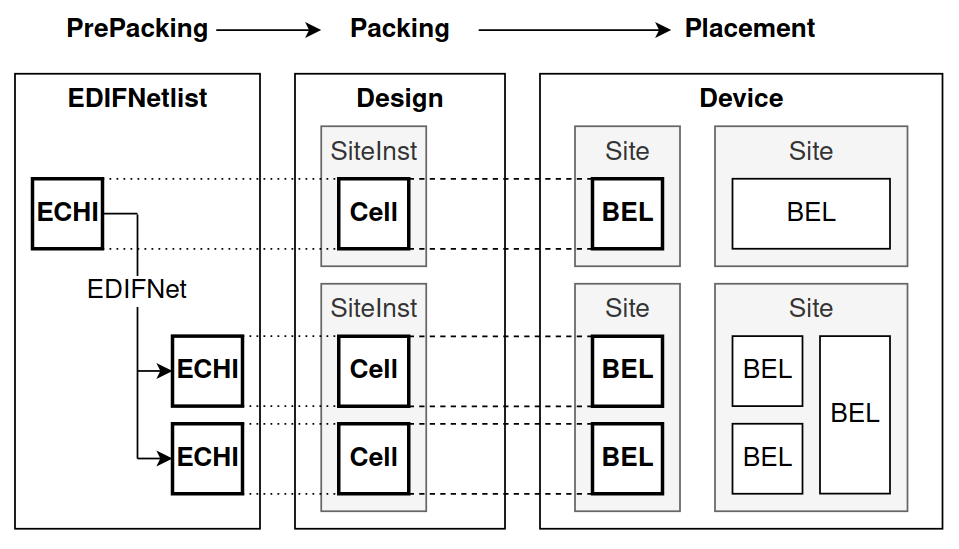
\includegraphics[width=0.9\columnwidth]{figures/edif_design_device.png}
    \captionof{figure}{Our placement workflow}
    \label{fig:edif_design_device}
}


\subsection{Prepacking}
\label{subsec:prepacking}


The first step in our placement flow is \textbf{prepacking}. 
Recall from the 7-Series architecture that there are certain multi-cell structures that must adhere to certain placements constraints to ensure legality, and by design, to minimize wirelength. 
The job of the prepacker is to traverse the raw EDIF netlist, detect these multi-cell structures, and consolidate these cells into clusters or groups of clusters that naturally reflect these placement constraints. 

Recall that \texttt{CARRY4} chains must necessarily be placed vertically and consecutively across a column of SLICEs in ascending order. 
Likewise, \texttt{DSP48E1} cascades must necessarily be placed vertically and consecutively across a column of DSP48E1 Sites in ascending order. 
A LUT-FF pair may be placed freely, but should be placed in the same lane within the same SLICE to minimize wirelength.

The raw EDIF netlist only tells us the list of nets and the cell ports that they connect to. 
It does not report the presence of any multi-cell structures (\texttt{CARRY4} chains, etc.). 
Thus, we must traverse the netlist to detect these multi-cell structures and store that structure information in a class we will call \texttt{PrepackedDesign}.

The code snippet in \ref{lst:carry_chains} shows how one can detect and collect these \texttt{CARRY4} chains using RapidWright. 
We first collect the cells in the design that are of type \texttt{CARRY4}, then iteratively traverse their Carry-Out (\texttt{CO}) to Carry-In (\texttt{CI}) nets to find incident \texttt{CARRY4} cells.
Each \texttt{CARRY4} chain has an anchor cell and a tail cell.
The anchor is found when the \texttt{CI} net connects to Ground (\texttt{GND}), while the tail is found when the \texttt{CO} port is null. 
We can further detect if there are \texttt{LUT}s or \texttt{FF}s connected to the \texttt{CARRY4} cell and store that information in a data structure we will call \texttt{CarryCellGroup} as defined in figure \ref{fig:substages}.
This will help us in knowing which cells can be packed together into the same \texttt{Site} in the subsequent stages. 

Similarly, \texttt{DSP48E1} cascades can be found and collected by traversing the \texttt{PCOUT} \texttt{ACOUT} and \texttt{BCOUT} nets.
\texttt{LUT-FF} pairs can be found by inspecting the LUT output (O) net and checking for FF input (DI) ports. 
We can bucket these LUT-FF pairs by finding the set of unique \texttt{CE} \texttt{SR} net pairs to know which group of LUT-FF pairs can be placed within the same \texttt{Site}. 
We detect and collect these multi-cellular structures and consolidate them into our \texttt{PrepackedDesign} object in preparation for the following Packing stage. 


\end{multicols}
{
    \centering
    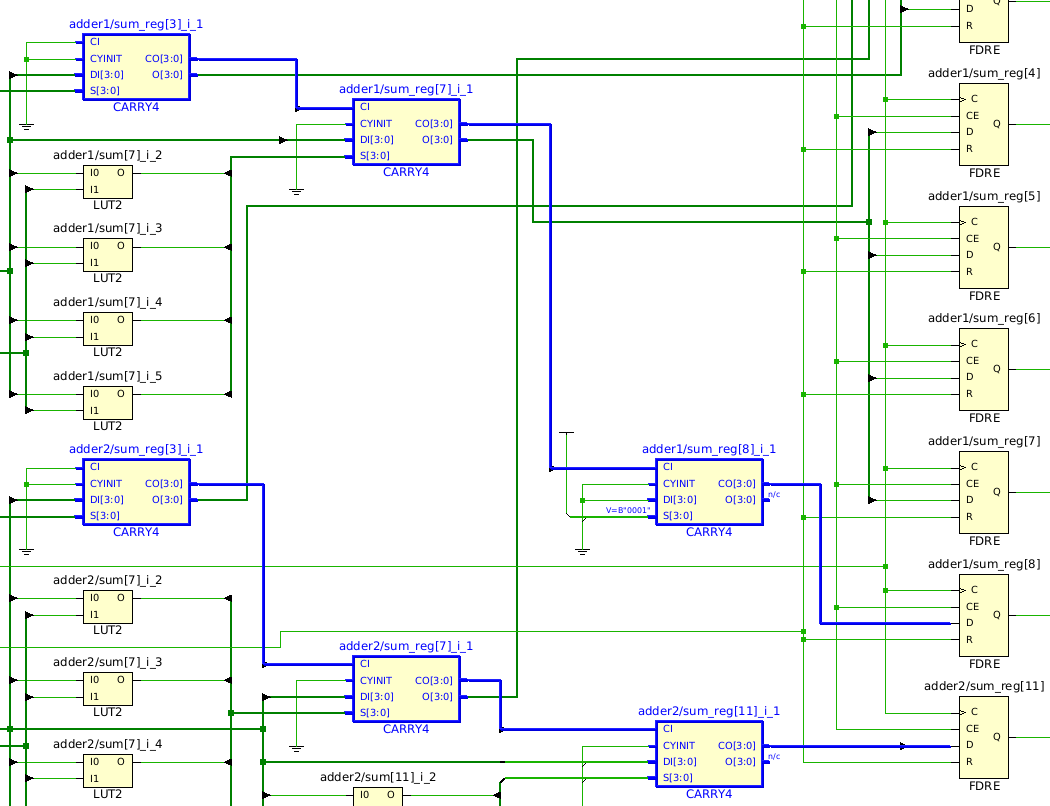
\includegraphics[width=0.8\columnwidth]{figures/carry_chain_traversal.png}
    \captionof{figure}{A netlist with two \texttt{CARRY4} chains, each of size 3}
    \label{fig:carry_chain_traversal}
}
\begin{multicols}{2}


\begin{lstlisting}[caption={Code Printout}]
Anchor Cell: adder2/sum_reg[3]_i_1, CellType: CARRY4
	Cell: adder2/sum_reg[7]_i_1, CellType: CARRY4
	Cell: adder2/sum_reg[11]_i_1, CellType: CARRY4
Anchor Cell: adder1/sum_reg[3]_i_1, CellType: CARRY4
	Cell: adder1/sum_reg[7]_i_1, CellType: CARRY4
	Cell: adder1/sum_reg[8]_i_1, CellType: CARRY4
\end{lstlisting}


\begin{lstlisting}[language=java, caption={Finding and storing carry chains.}, label={lst:carry_chains}]
Design design = Design.readCheckpoint("synth.dcp")
EDIFNetlist netlist = design.getNetlist();
List<EDIFCellInst> ecis = netlist.getAllLeafCellInstances();

// Select only the carry cells.
List<EDIFCellInst> carryCells = new ArrayList<>();
for (EDIFCellInst eci : ecis) {
    if (eci.getCellName().contains("CARRY4"))
        carryCells.add(eci);
}

// Find and remove carry chains until the list is empty
List<List<EDIFCellInst>> carryChains = new ArrayList<>();
while (!carryCells.isEmpty()) {
    // Arbitrarily set "currentCell" pointer to a cell in the list
    EDIFCellInst currentCell = carryCells.get(0);

    // Find this carry chain anchor.
    // Traverse the Carry-In (CI) to Carry-Out (CO) nets.
    // Anchor is found when net on the CI Port is Ground.
    while (true) {
        System.out.println(currentCell);
        // Access the CI port on this cell.
        EDIFPortInst sinkPort = currentCell.getPortInst("CI");
        // Access the net on this CI port.
        EDIFNet net = sinkPort.getNet();
        if (net.isGND()) {
            // Found this chain anchor!
            break;
        }
        // Get all ports on this net.
        List<EDIFPortInst> netPorts = net.getPortInsts();
        for (EDIFPortInst netPort : netPorts) {
            // Access the port belonging to another carry cell.
            EDIFCellInst sourceCell = netPort.getCellInst();
            if (sourceCell.getCellName().equals("CARRY4")) {
                // Move the "currentCell" pointer
                currentCell = sourceCell;
                break;
            }
        }
    }



    // Now we have the chain anchor as currentCell.
    // Now traverse in the opposite direction to find the chain tail.
    // Tail is found when the CO Port is null.
    // Collect the chain cells into an ordred list.
    List<EDIFCellInst> currentChain = new ArrayList<>();
    currentChain.add(currentCell);
    while (true) {
        System.out.println("while 2");
        EDIFPortInst sourcePort = currentCell.getPortInst("CO[3]");
        if (sourcePort == null) {
            // Found this chain's tail!
            break;
        }
        EDIFNet net = sourcePort.getNet();
        List<EDIFPortInst> netPorts = net.getPortInsts();
        for (EDIFPortInst netPort : netPorts) {
            EDIFCellInst sinkCell = netPort.getCellInst();
            if (netPort.getName().equals("CI") &&
                    sinkCell.getCellName().equals("CARRY4")) {
                currentCell = sinkCell;
                // Add the cell to the chain list.
                currentChain.add(currentCell);
                break;
            }
        }
    }
    System.out.println(currentChain.size());
    // Add currentChain to the list of chains
    carryChains.add(currentChain);
    // Remove currentChain from the list of cells
    carryCells.removeAll(currentChain);
} // end while()

// Print out the carry chains. 
for (List<EDIFCellInst> chain : chains) {
    for (int i = 0; i < chain.size(); i++) {
        EDIFCellInst carry = chain.get(i);
        if (i == 0) {
            writer.write("\nAnchor Cell: " + carry.getName() + 
                ", CellType: " + carry.getCellName());
        } else {
            writer.write("\n\tCell: " + carry.getName() + 
                ", CellType: " + carry.getCellName());
        }
    }
}
\end{lstlisting}




\subsection{Packing}
\label{subsec:packing}
Now that we have our \texttt{PrepackedDesign} object keeping track of multi-cell structures on the \texttt{edif} level, we can start packing them into \texttt{SiteInst} objects on the \texttt{design} level. 
A \texttt{SiteInst} object can be created and its BELs populated by existing \texttt{EDIFHierCellInst} objects. 
A \texttt{SiteInst} is necessarily placed on a specific \texttt{Site} upon creation. 
Thus, the packer necessarily gives all \texttt{SiteInst}s an initial placement before randomization via simulated annealing in the following placement stage. 
In packing, will simply assign \texttt{SiteInst}s pseudorandomly onto device \texttt{Site}s on a first-come-first-serve basis by coordinate order (first SiteInst onto \texttt{SLICEL\_X0Y0}, second \texttt{SiteInst} onto \texttt{SLICEL\_X0Y1}, etc.). 


\end{multicols}
\begin{lstlisting}[caption=\texttt{SiteInst} construction and BEL population.]
Constructor: 
    SiteInst(String name, Design design, SiteTypeEnum type, Site site)

Usage:
    SiteInst si = new SiteInst(<name>, <design>, <type>, <site>);
    si.createCell(<EDIFHierCellInst>, <BEL>);
\end{lstlisting}




\begin{lstlisting}[language=java, caption={Packing DSPCascades into \texttt{DSP48E1} \texttt{SiteInst}s.}, label={lst:carry_chains}]
private List<List<SiteInst>> packDSPCascades(List<List<EDIFHierCellInst>> EDIFDSPCascades) throws IOException {
    List<List<SiteInst>> siteInstCascades = new ArrayList<>();
    writer.write("\n\nPacking DSP Cascades... (" + EDIFDSPCascades.size() + ")");
    for (List<EDIFHierCellInst> cascade : EDIFDSPCascades) {
        List<SiteInst> siteInstCascade = new ArrayList<>();
        // each DSP tile has 2 DSP sites on the Zynq 7000
        writer.write("\n\tCascade Size: (" + cascade.size() + "), Cascade Anchor: "
                + cascade.get(0).getFullHierarchicalInstName());
        // Select a Site location on the device. 
        Site anchorSite = selectDSPAnchorSite(cascade.size());
        SiteTypeEnum siteType = SiteTypeEnum.DSP48E1;
        for (int i = 0; i < cascade.size(); i++) {
            writer.write("\n\t\tPlacing DSP: " + cascade.get(i).getFullHierarchicalInstName());
            Site site = (i == 0) ? anchorSite
                    : device.getSite("DSP48_X" + anchorSite.getInstanceX() + "Y" + (anchorSite.getInstanceY() + i));
            // Create the SiteInst object
            SiteInst si = new SiteInst(cascade.get(i).getFullHierarchicalInstName(), design, siteType, site);
            // Populate the SiteInst with a DSP Cell. 
            si.createCell(cascade.get(i), si.getBEL("DSP48E1"));
            occupiedSites.get(siteType).add(site);
            availableSites.get(siteType).remove(site);
            si.routeSite();
            siteInstCascade.add(si);
        }
        siteInstCascades.add(siteInstCascade);
    }
    return siteInstCascades;
} // end packDSPCascades()
\end{lstlisting}

\begin{lstlisting}[language=java, caption={Packing LUTGroups into \texttt{SLICEL} \texttt{SiteInst}s}]
protected String[] LUT6_BELS = new String[] { "A6LUT", "B6LUT", "C6LUT", "D6LUT" };

private List<SiteInst> packLUTGroups(List<List<EDIFHierCellInst>> LUTGroups) throws IOException {
    List<SiteInst> LUTSiteInsts = new ArrayList<>();
    writer.write("\n\nPacking LUT Groups...");
    for (List<EDIFHierCellInst> group : LUTGroups) {
        Site selectedSite = selectCLBSite();
        SiteInst si = new SiteInst(group.get(0).getFullHierarchicalInstName(), design,
                selectedSite.getSiteTypeEnum(), selectedSite);
        for (int i = 0; i < group.size(); i++) {
            si.createCell(group.get(i), si.getBEL(LUT6_BELS[i]));
        }
        si.routeSite();
        // for whatever reason, this does not activate DUSED PIP for
        si.addSitePIP(si.getSitePIP("DUSED", "0"));
        si.addSitePIP(si.getSitePIP("CUSED", "0"));
        si.addSitePIP(si.getSitePIP("BUSED", "0"));
        si.addSitePIP(si.getSitePIP("AUSED", "0"));
        LUTSiteInsts.add(si);
    }
    return LUTSiteInsts;
} // end packLUTGroups()
\end{lstlisting}
\begin{multicols}{2}



\subsection{Placement}
    \label{subsec:placement}
    Up until now we have only organized the logical \texttt{EDIFCellInst}s into \texttt{SiteInst}s. 
    This is where simulated annealing actually begins where we actually place the \texttt{SiteInst}s onto physical \texttt{Site}s on the \texttt{device} level. 

